\documentclass{beamer}
\mode<presentation>{}

\usepackage{amsmath}
\usepackage{graphicx}
\usepackage{listings}
\usepackage{color}

\graphicspath{ {/Users/matthewdrury/Presentations/boosting-presentation-for-galvanize/plots/} }

\AtBeginSection[]{
  \begin{frame}
  \vfill
  \centering
  \begin{beamercolorbox}[sep=8pt,center,shadow=true,rounded=true]{title}
    \usebeamerfont{title}\insertsectionhead\par%
  \end{beamercolorbox}
  \vfill
  \end{frame}
}

\definecolor{mygreen}{rgb}{0,0.6,0}
\definecolor{mygray}{rgb}{0.5,0.5,0.5}
\definecolor{mymauve}{rgb}{0.58,0,0.82}

% Code formatting stuff.
\lstset{ %
  backgroundcolor=\color{white},   % choose the background color; you must add \usepackage{color} or \usepackage{xcolor}
  basicstyle=\scriptsize,          % the size of the fonts that are used for the code
  breakatwhitespace=false,         % sets if automatic breaks should only happen at whitespace
  breaklines=true,                 % sets automatic line breaking
  captionpos=b,                    % sets the caption-position to bottom
  commentstyle=\color{mygreen},    % comment style
  deletekeywords={...},            % if you want to delete keywords from the given language
  escapeinside={\%*}{*)},          % if you want to add LaTeX within your code
  extendedchars=true,              % lets you use non-ASCII characters; for 8-bits encodings only, does not work with UTF-8
  keepspaces=true,                 % keeps spaces in text, useful for keeping indentation of code (possibly needs columns=flexible)
  keywordstyle=\color{blue},       % keyword style
  language=Octave,                 % the language of the code
  otherkeywords={*,...},           % if you want to add more keywords to the set
  numbers=none,                    % where to put the line-numbers; possible values are (none, left, right)
  numbersep=5pt,                   % how far the line-numbers are from the code
  numberstyle=\tiny\color{mygray}, % the style that is used for the line-numbers
  showspaces=false,                % show spaces everywhere adding particular underscores; it overrides 'showstringspaces'
  showstringspaces=false,          % underline spaces within strings only
  showtabs=false,                  % show tabs within strings adding particular underscores
  stepnumber=2,                    % the step between two line-numbers. If it's 1, each line will be numbered
  stringstyle=\color{mymauve},     % string literal style
  tabsize=2,	                   % sets default tabsize to 2 spaces
  title=\lstname                   % show the filename of files included with \lstinputlisting; also try caption instead of title
}


\DeclareMathOperator*{\argmin}{arg\,min}
\DeclareMathOperator*{\bias}{bias}
\DeclareMathOperator*{\var}{var}
\DeclareMathOperator*{\tr}{tr}
\DeclareMathOperator*{\pd}{pd}
I\DeclareMathOperator*{\goesto}{\rightarrow}
%\DeclareMathOperator*{\implies}{\Rightarrow}

\title{Boosting}
\author{Matthew Drury}

\begin{document}
%
\begin{frame}
  \titlepage
\end{frame}
%
\begin{frame}
  Boosting encompasses an entire family highly successful learning algorithms.
\end{frame}
%
\begin{frame}
Boosting can adapt itself effortlessly to very non-linear objectives
  \only<1>{
    \begin{figure}
      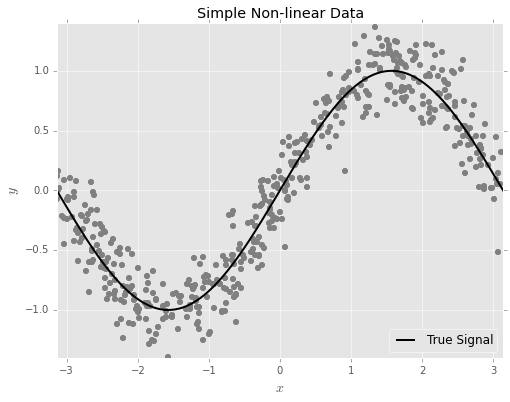
\includegraphics[scale=0.50]{sin-with-data}
    \end{figure}
   }
   \only<2>{
    \begin{figure}
      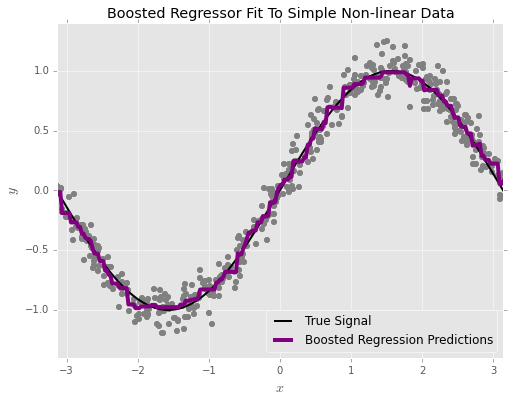
\includegraphics[scale=0.50]{sin-with-data-and-booster}
    \end{figure}
   }
   \only<3>{
    \begin{figure}
      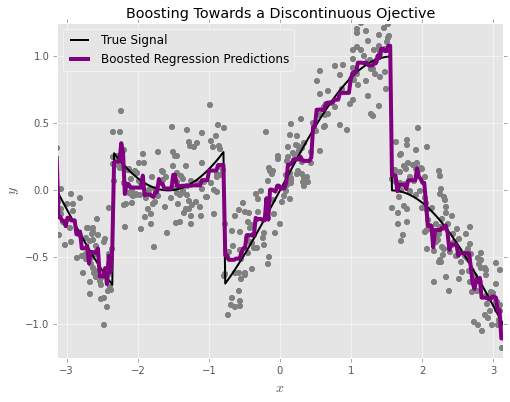
\includegraphics[scale=0.50]{broken-sin-with-booster}
    \end{figure}
   }
\end{frame}
%
\begin{frame}
Boosting accomplishes this by \textit{growing the model gradually}
  \begin{figure}
    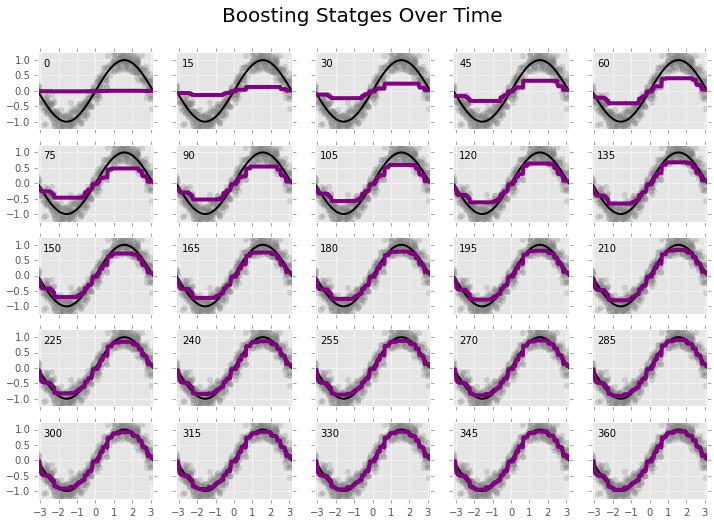
\includegraphics[scale=0.40]{boosting-over-time-multiple-plots}
  \end{figure}
\end{frame}
%
\begin{frame}
At each stage of the growth, the next model is built as an adjustment to the previous model
  \begin{figure}
    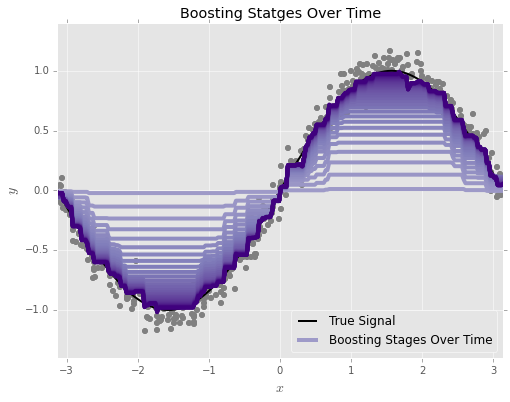
\includegraphics[scale=0.50]{boosting-over-time-single-plot}
  \end{figure}
\end{frame}
%
\begin{frame}

\only<2->{  
\textbf{Compared to}:\\~\\
}

\only<1>{
\textbf{Boosting}: \\~\\
Lowers variance by growing the model slowly over time (along with a few other tricks).\\~\\

Lowers bias by stacking many non-parametric models into the final result.
}

\only<2>{
\textbf{Linear Models}: \\~\\
Lowers variance by using a regularization penalty.\\~\\

Lowers bias by including more features.
}

\only<3>{
\textbf{SVM}: \\~\\
Lowers variance by maximizing the margin between positive and negative cases.\\~\\ 

Lowers bias by using a kernel, which projects the data into a very high dimensional space.
}

\only<4>{
\textbf{Random Forest}: \\~\\

Lowers variance by growing many learners on different subsamples of the data and predictors, then averaging them.\\~\\

Lowers bias by growing really big trees.
}

\end{frame} % Introduction
\section{Outline of the Lesson}
%
\begin{frame}
\textbf{Agenda:}
 
  \begin{itemize}
    \item Introduction
    \item You Could Have Invented Gradient Boosting
    \item Practical Gradient Boosted Regression
    \item Interpreting Gradient Boosted Regression
    \item Boosting for Classification.
    \item Drawbacks of Boosting
  \end{itemize}

\end{frame}
%
\begin{frame}
\textbf{Objectives:}

  \begin{itemize}
    \item Understand the conceptual foundation of Boosting
    \item Understand the algorithm's hyperparameters, and how to tune them.
    \item Understand some basic strategies for interpreting a booster.
    \item Understand the drawbacks of boosting.
    \item Be aware of the possibility of creating your own loss function.
  \end{itemize}
  
\end{frame} % Outline and Goals
\section{You Could Have Invented Gradient Boosting}
%
\begin{frame}
Let's start with our usual basic setup.\\~\\

$\{ x_i, y_i \}$ is a data set, where $i$ indexes the samples we have available for training our model.\\~\\

Each $x_i$ may be a vector, in which case I'll refer to it's components (if needed) as $x_{ij}$.
\end{frame}
%
\begin{frame}
Our goal is to construct a function $f$ so that

$$ y_i \approx f(x_i) \ \text{for all} \ i $$

\end{frame}
%
\begin{frame}
\textbf{Question:} What should the domain of $f$ be?
\end{frame}
%
\begin{frame}
\textbf{Degenerate Choice:} 

$$\text{Domain}(f) = \{x_i\}$$.

That is, let's only attempt to define $f$ on our training samples.
\end{frame}
%
\begin{frame}
\begin{center}
"But Matt.  This is silly.  The answer is obvious."
\end{center}

$$ \textbf{Define:} \ f(x_i) = y_i $$
\end{frame}
%
\begin{frame}
\textbf{True}.\\~\\

But let's try to derive this in a creative way.
\end{frame}
%
\begin{frame}

\only<1>{
\textbf{Recall}: Gradient descent is a general purpose algorithm for optimizing any objective function $L(x)$.\\~\\

  \begin{center}
    \textit{How does this go?}
  \end{center}
}

\only<2>{
\textbf{Algorithm:} Gradient Descent to Minimize a function $L$.\\~\\

\textbf{Inputs:} A function $f$.

\textbf{Outputs:} A point $x_{\text{optim}}$ that minimizes $f$. \\~\\

\begin{itemize}
  \item Compute $\nabla L(x)$ somehow, on paper is good.
  \item Initialize $x_0 = 0$ (arbitrary, there may be more principled choices).
  \item Iterate until convergence: \begin{itemize}
    \item Set $x_{i+1} = x_i - \nabla L(x_i)$.
  \end{itemize}
\end{itemize}
}

\end{frame}
%
\begin{frame}
Let's focus on a \textit{single point in our domain}, and try to minimize the classic squared error loss function

$$ L(f, y) = \frac{1}{2} (y - f)^2 $$

Here $f$ is not a function yet, it is just a number.
\end{frame}
%
\begin{frame}
Initialize $f$ to the average value of $y_i$

$$ f_0 = \frac{1}{N} \sum_i y_i $$
\end{frame}
%
\begin{frame}
Compute the gradient with respect to $f$ by hand

$$ \nabla_{f} (f, y) = \frac{\partial}{\partial f} \left( \frac{1}{2} (y - f)^2 \right) = f - y $$
\end{frame}
%
\begin{frame}
...and apply the update rule

$$ f_1 = f_0 - \nabla_{f} (f_0, y) = f_0 - (f_0 - y) = y $$
\end{frame}
%
\begin{frame}
So this (admittedly quite bizarre) application of gradient descent immediately recovers the correct solution

$$ f(x_i) = y_i $$

for every data point.
\end{frame}
%
\begin{frame}

\begin{center}
\textbf{Question:}\\~\\

What is stopping up from applying this scheme in the more realistic situation where we want to construct a function $f$ with domain $\mathbb{R}^n$ so that
\end{center}

$$ f(x_i) \approx y_i $$
\end{frame}
%
\begin{frame}
The \textbf{first step works}, we can certainly define $f_0$ to be a constant function

$$ f_0(x) = \frac{1}{N} \sum_i y_i \ \text{for all} \ x \in \mathbb{R}^n $$
\end{frame}
%
\begin{frame}
The \textbf{update step fails}.\\~\\

We cannot evaluate the gradient at any point where we have not observed a value of $y$.

$$ \nabla_f (f, y) = f - y $$
\end{frame}
%
\begin{frame}

\begin{center}
{\huge We need to extend the gradient to points where we have not observed a value of $y$.}
\end{center}

\end{frame}

%
\begin{frame}
\textbf{Fundamental Idea Of Gradient Boosting:}\\~\\

Replace the response $y$ in our dataset with the \textbf{gradient of the loss evaluated at} $y$

$$ \{x_i, \nabla_f L(f_0(x_i), y_i) \} = \{x_i, f_0(x_i) - y_i \} $$

Then, fit a model to this new \textbf{working response}.\\~\\

The \textbf{predictions from this model} can be viewed as an (approximate) extension of the gradient to all of $\mathbb{R}^n$.

\end{frame}
%
\begin{frame}
\textbf{Algorithm:} Gradient Boosting to Minimize Sum of Squared Errors.\\~\\

\textbf{Inputs:} A data set $\{ x_i, y_i \}$.

\textbf{Returns:} A function $f$ such that $f(x_i) \approx y_i$.

\begin{itemize}
  \item Initialize $f_0(x) = \frac{1}{N} \sum_i y_i$.
  \item Iterate (parameter $k$) until satisfied: \begin{itemize}
    \item Create the working data set $W_k = \{ x_i, f_k(x_i) - y_i \}$.
    \item Fit a decision tree to $W_k$, minimizing least squares (though most anything would work here).  Call this tree $T_k$.
    \item Set $f_{k+1}(x) = f_{k}(x) - T_{k}(x)$. 
  \end{itemize}
  \item Return $f_{\text{max}}(x) = f_0(x) - T_1(x) - T_2(X) - \cdots - T_{\text{max}}(x)$.
\end{itemize}
\end{frame}
%
\begin{frame}
\textbf{Comments:}

\only<2->{
\begin{itemize}
  \item We didn't \textit{have} to use decision trees, literally anything would work.
}
\only<3->{
  \item Just like in other algorithms, we can introduce a \textit{learning rate} to make the gradient descent more robust
  $$ x_{i+1} = x_i - \lambda \nabla L(x_i) $$
This is particularly important in boosting, to prevent overfitting.
}
\only<4->{
  \item We could have fit the tree to the negative gradient, which would have resulted in the more aesthetically appealing
  $$ f_{\text{max}}(x) = f_0(x) + T_1(x) + T_2(X) + \cdots + T_{\text{max}}(x) $$
}
\only<2->{
\end{itemize}
}
\end{frame}




 % You Could Have Invented Gradient Boosting
\section{Practical Gradient Boosted Regression}
%
\begin{frame}[fragile]
Scikit-learn includes the gradient boosted regression algorithm in the \texttt{ensembles} module\\~\\

\begin{lstlisting}[language=python]
from sklearn.ensemble import GradientBoostedRegressor
\end{lstlisting}

\end{frame}
%
\begin{frame}[fragile]

\texttt{GradientBoostingRegressor} has many knobs to turn.\\~\\

\begin{lstlisting}[language=python]
GradientBoostingRegressor(loss='ls', 
                          learning_rate=0.1, 
                          n_estimators=100, 
                          subsample=1.0, 
                          min_samples_split=2, 
                          min_samples_leaf=1, 
                          min_weight_fraction_leaf=0.0,
                          max_depth=3,
                          ...)
\end{lstlisting}

\end{frame}
%
\begin{frame}[fragile]
A \texttt{GradientBoostingRegressor} object is fit in the same way as every other leaning model in sklearn\\~\\

\begin{lstlisting}[language=python]
model = GradientBoostingRegressor()
model.fit(X, y)
\end{lstlisting}

\end{frame}
%
\begin{frame}[fragile]
The \texttt{predict} method returns predictions on new data\\~\\

\begin{lstlisting}[language=python]
preds = model.predict(X_new)
\end{lstlisting}

Especially useful is the iterator \texttt{staged\_predict} which creates predictions from models created by truncating series of trees\\~\\

\begin{lstlisting}[language=python]
for preds in model.staged_predict(X_new):
    # Do something interesting, see the plots below.
\end{lstlisting}

\end{frame}
%
\begin{frame}[fragile]
The most important options to \texttt{GradientBoostedRegressor} are

\begin{itemize}
  \item \texttt{loss} controls the loss function to minimize.  \texttt{ls} is the least squares minimization algorithm we discussed in the previous section.
  \item \texttt{n\_estiamtors} is how many boosting stages to compute, i.e. how many regression trees to grow.
  \item \texttt{learning\_rate} is the learning rate for the gradient update.
  \item \texttt{max\_depth} controls how deep to grow each individual tree.
  \item \texttt{subsample} allows to fit each tree on a random sample of the training data (like bagging in random forests).
\end{itemize}

\end{frame}
%
\begin{frame}{Tuning the Number of Estimators}

As more and more trees are added to the model the training set error will be driven down monotonically, but the same is not true for the testing error

  \begin{figure}
    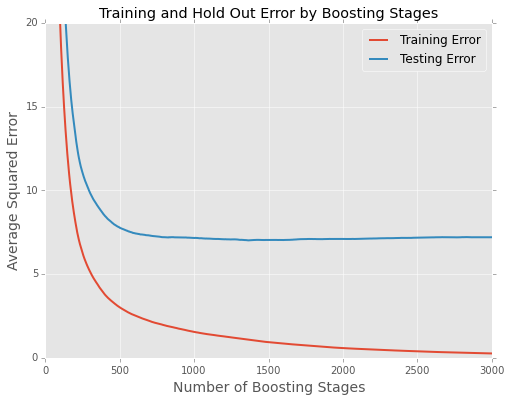
\includegraphics[scale=0.45]{training-and-testing-error}
  \end{figure}

\end{frame}
%
\begin{frame}

  \begin{figure}
    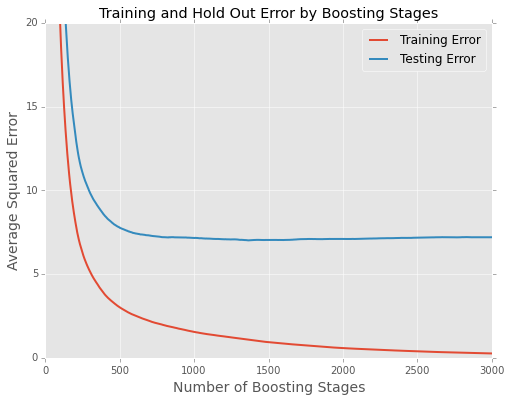
\includegraphics[scale=0.45]{training-and-testing-error}
  \end{figure}

This means that it is essential to determine the proper number of trees to grow, as too many may lead to overfitting

\end{frame}
%
\begin{frame}
One way to tune the numer of trees is to make use of a validation set, held out from both training and testing

  \begin{figure}
    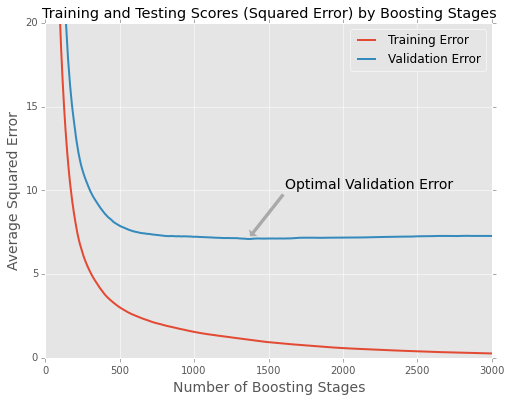
\includegraphics[scale=0.45]{training-and-testing-error-with-optima}
  \end{figure}
  
\end{frame}
%
\begin{frame}[fragile]
The \texttt{loss\_} method is important here, it allows us to compute the loss function on held out data\\~\\

\begin{lstlisting}[language=python]
validation_loss = np.zeros(model.get_params('n_estimators'))
for i, preds in enumerate(model.staged_predict(X_new)):
    validation_loss[i] = model.loss_(preds, y_new)
    
optimal_tree = np.argmin(validation_loss)
optimal_loss = validation_loss[optimal_tree]
\end{lstlisting}

\end{frame}
%
\begin{frame}
Another way to choose the optimal number of trees is to replace the validation set with cross validation

  \begin{figure}
    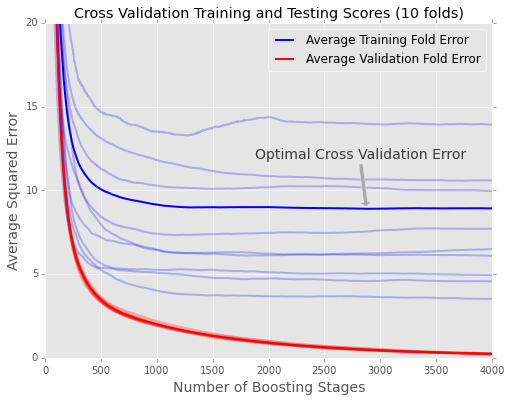
\includegraphics[scale=0.45]{training-and-testing-cv-error}
  \end{figure}
  
\end{frame}
%
\begin{frame}

  \begin{figure}
    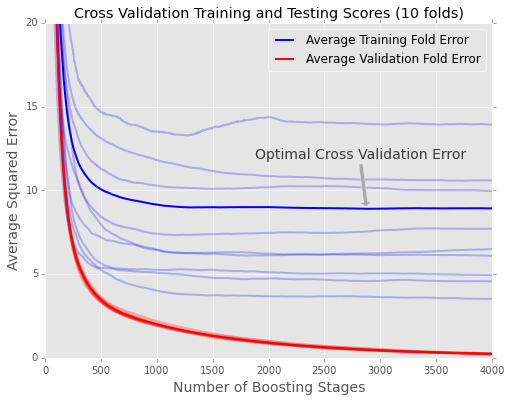
\includegraphics[scale=0.45]{training-and-testing-cv-error}
  \end{figure}
  
We generally choose the number of trees minimizing the \textit{average} out validation fold error.

\end{frame}
%
\begin{frame}{Tuning the Learning Rate}

The learning rate allows us to grow our boosted model slowly.\\~\\

A large learning rate will cause the model to fit hard to the training data, which creates a \textit{high variance} situation.\\~\\

A smaller learning rate reduces the boosted models sensitivity to the training data.\\~\\

\end{frame}
%
\begin{frame}
Decreasing the learning rate reduces how fast the booster drives down the training error rate
  \begin{figure}
    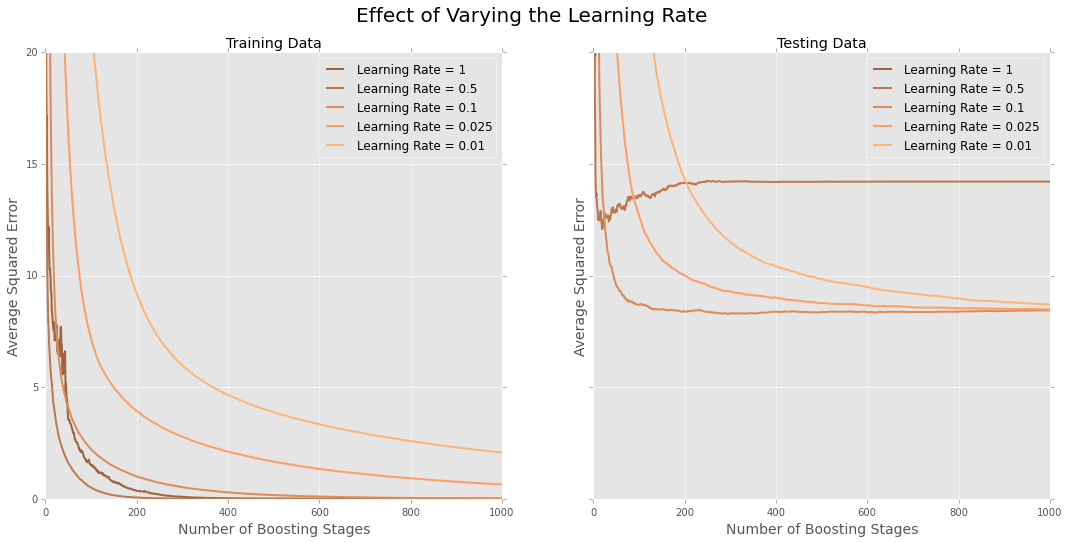
\includegraphics[scale=0.30]{varying-learning-rate-error}
  \end{figure}
  
\end{frame}
%
\begin{frame}
On the other hand, a smaller learning rate means more trees are needed to reach the optimal point

  \begin{figure}
    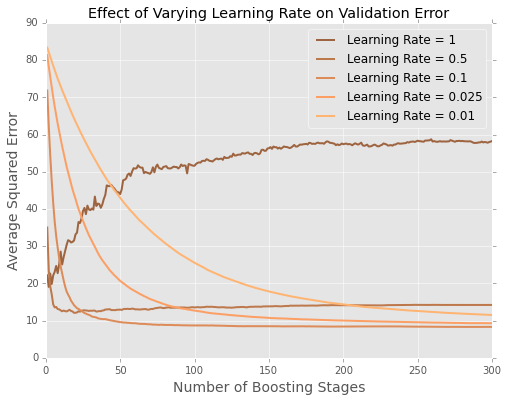
\includegraphics[scale=0.50]{varying-learning-rate-error-testing-zoom-start}
  \end{figure}
  
\end{frame}
%
\begin{frame}
In general, a smaller learning rate eventually (over enough time) results in a superior model

  \begin{figure}
    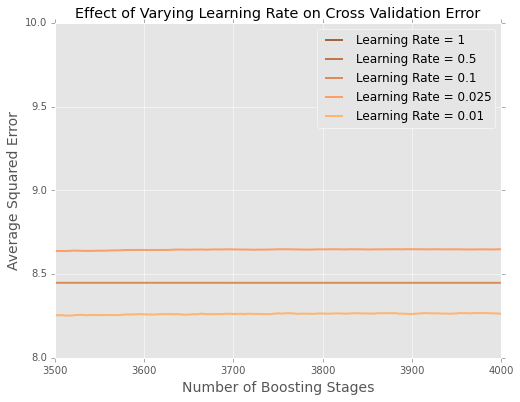
\includegraphics[scale=0.50]{varying-learning-rate-error-testing-zoom-end}
  \end{figure}
  
\end{frame}
%
\begin{frame}
\textbf{Strategy for Learning Rate}:

\begin{itemize}
  \item In the initial exploratory phases of modeling, set the learning rate to some large value, say $0.1$.  This allows you to iterate through ideas quickly.
  \item When tuning other parameters using grid search, decrease the learning rate to a more sensible value, $0.01$ works well.
  \item When fitting the \textit{final} production model, set the learning rate to a very small value, $0.001$ or $0.0005$, smaller is better.
\end{itemize}

\end{frame}
%
\begin{frame}

Run the final model overnight!  It will fit while you are sleeping!\\~\\

Make sure you've written all your analysis code up front, based on your initial models.  Then all that's left is to run your final model through and see your final statistics.
\end{frame}
%
\begin{frame}{Tuning the Tree Depth}
A larger tree depth allows the model to capture deeper interactions between the predictors, resulting in lower bias.

  \begin{figure}
    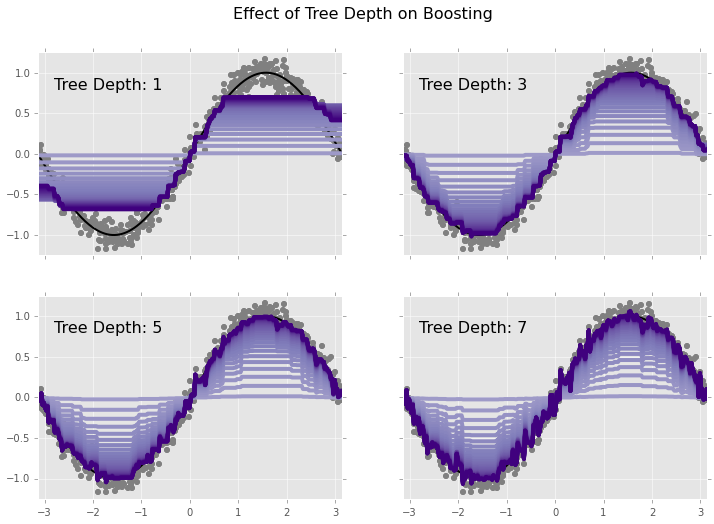
\includegraphics[scale=0.3]{sin-changing-depth}
  \end{figure}

Unfortunately, a deeper tree depth also causes the model to fit faster, increasing the variance and somewhat combating the effect of the learning rate.
\end{frame}
%
\begin{frame}
It's never obvious up front what tree depth is best for a given problem, so a grid search is needed to determine the best value

  \begin{figure}
    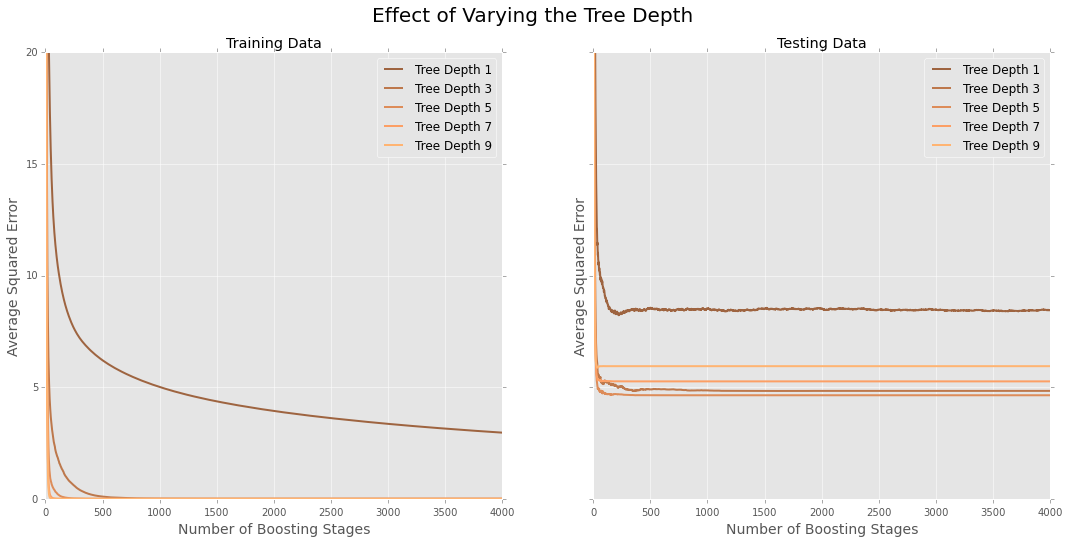
\includegraphics[scale=0.50]{varying-tree-depth-error}
  \end{figure}
  
\end{frame}
%
\begin{frame}
\textbf{Strategy for Tree Depth}:

Tune with a grid search and cross validation.
  
\end{frame}
%
\begin{frame}
It's never obvious up front what tree depth is best for a given problem, so a grid search is needed to determine the best value

  \begin{figure}
    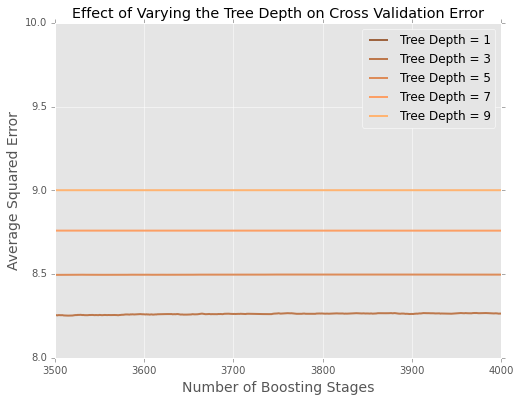
\includegraphics[scale=0.50]{varying-tree-depth-error-zoom}
  \end{figure}
  
\end{frame}
%
%
\begin{frame}{Tuning the Subsample Rate}
The \texttt{subsample} parameter allows one to train each tree on a subsample of the training data.\\~\\

This is similar to bagging in the random forest algorithms, and has the same result: it lowers the variance of the resulting model.
\end{frame}
%
\begin{frame}
Not subsampling at all, or over subsampling are both bad ideas

  \begin{figure}
    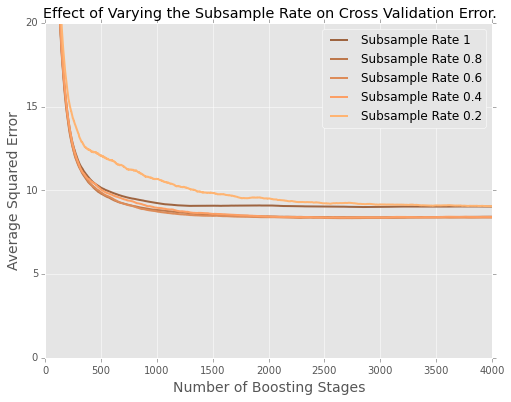
\includegraphics[scale=0.50]{varying-subsample-rate-error}
  \end{figure}
 
\end{frame}
%
\begin{frame}
Between these two extremes, different levels of subsampling generally give the same performance

  \begin{figure}
    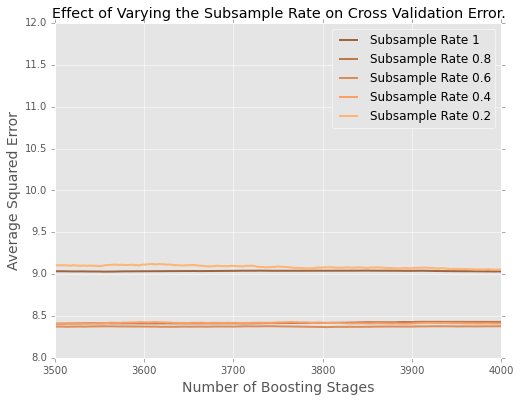
\includegraphics[scale=0.50]{varying-subsample-rate-error-zoom-end}
  \end{figure}
  
\end{frame}
%
\begin{frame}
\textbf{Strategy For Subsample:}

Set to $0.5$, it almost always works well.
\end{frame}

   % Practical Gradient Boosted Regression
\section{Interpreting Gradient Boosting}

\begin{frame}
Gradient boosting models, while offering massive predictive power, are very complex and hard to interpret.
\end{frame}
%
\begin{frame}
There are two high level summarization techniques that are very popular, and can help understand the high level content of the model and diagnose issues

\begin{itemize}
  \item \textbf{Relative Variable Importance}: Measures the amount a predictor "participates" in the model fitting procedure.
  \item \textbf{Partial Dependence Plots}: Are analogous to parameter estimates in linear regressions, they summarize the effect of a single predictor while controlling for the effect of all others.
\end{itemize}
\end{frame}
%
\begin{frame}{Relative Variable Importance}
The concept here is the same as in random forest.\\~\\

\only<2->{
Each time we grow a tree, we keep track of how much the error metric decreases at each split, and allocate that decrease to a predictor.\\~\\
}

\only<3->{
The importance of a predictor \texttt{in a tree} is the total amount the error metric decreased over all splits on that predictor\\~\\
}

\only<4->{
The importance of a predictor in the boosted model is the \texttt{average} importance of the predictor over all the trees.
}

\end{frame}
%
\begin{frame}
It is traditional to normalize the importances so that they sum to $100$.

  \begin{figure}
    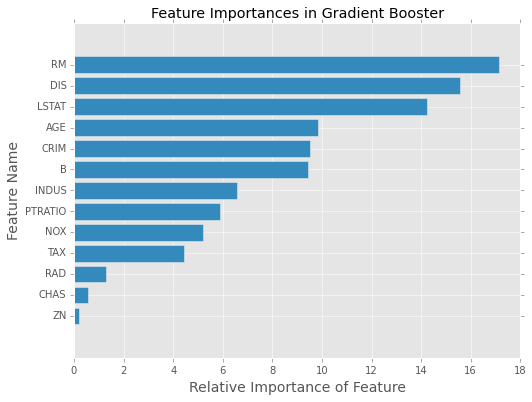
\includegraphics[scale=0.45]{feature-importances}
  \end{figure}
  
\end{frame}
%
\begin{frame}
\textbf{Comments:}\\~\\

\begin{itemize}

\only<1>{
    \item The name "feature importances" is pretty awful.  It invites misinterpretation.  
    \begin{center}
    \textit{Don't reason about things from the names they have been given, make sure the statistic actually answers your question}.
    \end{center}
}

\only<2>{
    \item If your model contains both numeric and binary predictors, the importance metric is biased to assign higher values to the numeric predictors.  Try not to compare feature importances across these two classes.
}

\only<3>{
    \item Feature importance rankings can have very high variance.  Make sure
    any important conclusions are robust to different RNG seeds and training sets.
}

\only<4>{
    \item Make sure your model only includes trees \textit{up to the optimal point}.  Otherwise you'll allocate importance to overfitting.
}

\only<5>{
    \item Dominant features should be treated with suspicion.  They can often be a sign of data leakage.
}
\end{itemize}
\end{frame}
%

\begin{frame}{Partial Dependence Plots}

Visualizations of the effect of a single predictor, averaging out the effects of all the rest

  \begin{figure}
    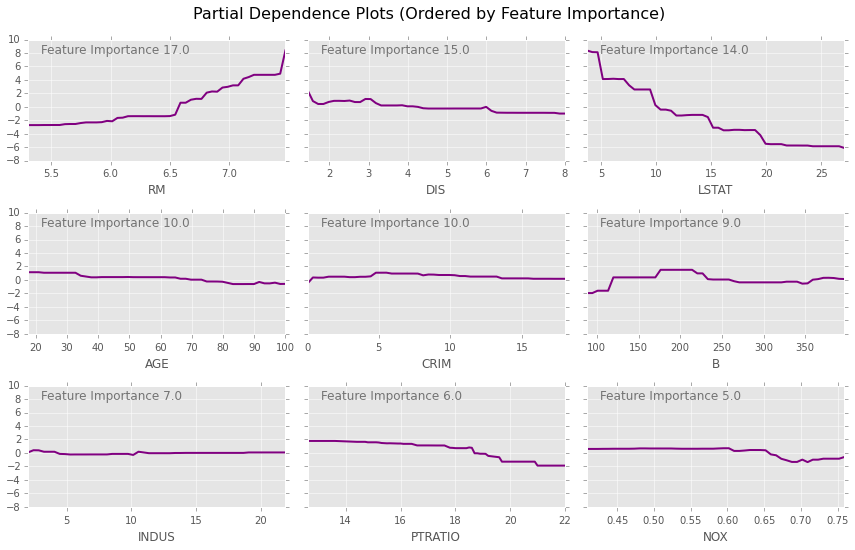
\includegraphics[scale=0.33]{patial-dependence-plots}
  \end{figure}

\end{frame}
%
\begin{frame}
In symbols:

$$ \pd_j(x) = \frac{1}{N} \sum_i f(\overbrace{x_{i1}, x_{i2}}^{\text{The training data points}}, \ldots, \overbrace{x}^{\text{The j'th spot}}, \ldots, x_{iM}) $$
\end{frame}
%
\begin{frame}
By varying the values of two predictors, we can draw partial dependence plots in higher dimensions

  \begin{figure}
    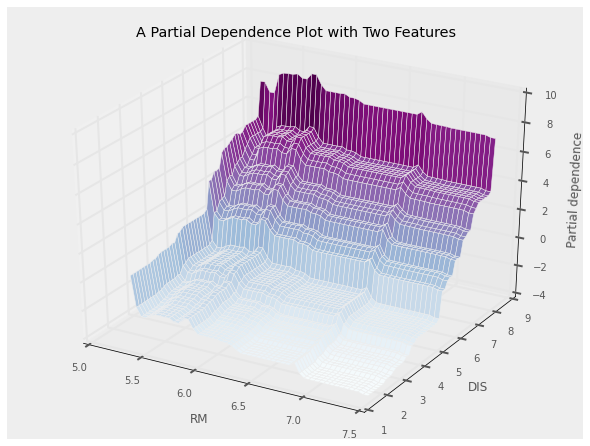
\includegraphics[scale=0.45]{patial-dependence-plot-two-features}
  \end{figure}
 
\end{frame}
%
\begin{frame}
\textbf{Question:} Does it look like any trees split on \textit{both} RM and DIS?

  \begin{figure}
    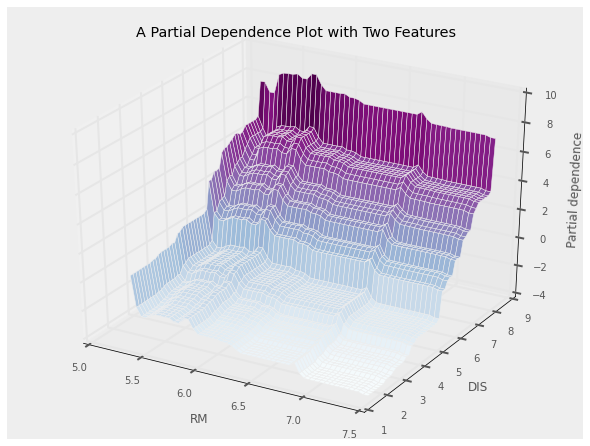
\includegraphics[scale=0.45]{patial-dependence-plot-two-features}
  \end{figure}
 
\end{frame}
%
\begin{frame}
\textbf{Question:} What about AGE and DIS?

  \begin{figure}
    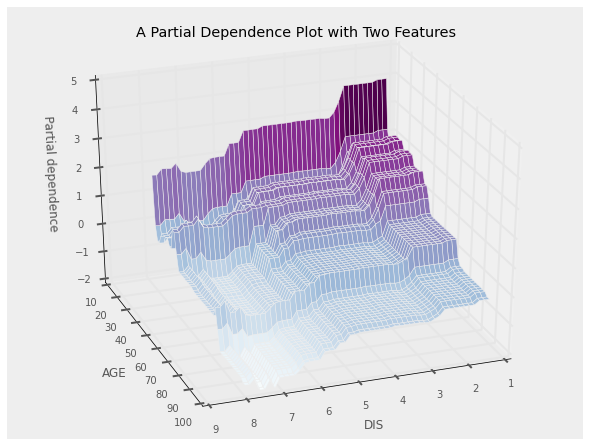
\includegraphics[scale=0.45]{patial-dependence-plot-two-features-with-interaction}
  \end{figure}
 
\end{frame}
 % Partial Dependence Plots + Variable Importance
\section{Other Gradient Boosting Algorithms}

\begin{frame}
The last great feature of Gradient Boosting is that it generalizes easily to other loss functions.
\end{frame}
%
\begin{frame}
We will discuss two generalizations:

\begin{itemize}
  \item \textbf{Gradient Boosted Logistic Regression}: Minimizes the binomial deviance (logistic log likelihood) loss function.
  \item \textbf{AdaBoost}: Minimizes a custom classification loss.
\end{itemize}

It is important to say: \textit{There are many more possibilities}!
\end{frame}
%
\begin{frame}{Gradient Boosted Logistic Regression}
We want to generalize our boosting algorithm to also solve \textit{classification} problems. 

$$ y \in  \{0, 1\} $$

We want to estimate $ f(x) = Pr(y = 1 \mid x) $.
\end{frame}
%
\begin{frame}
For example, here is a complex classification problem

  \begin{figure}
    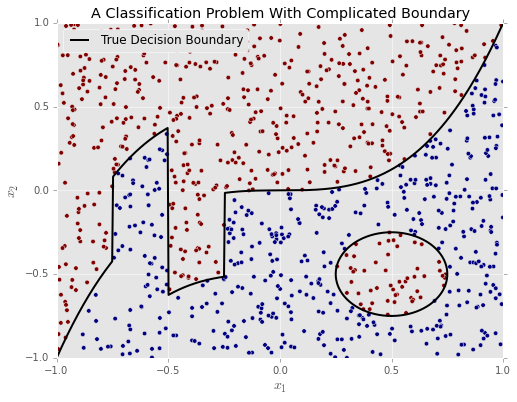
\includegraphics[scale=0.45]{classification-boundary-with-data}
  \end{figure}

\end{frame}
%
\begin{frame}
How would you solve this with standard logistic regression?

  \begin{figure}
    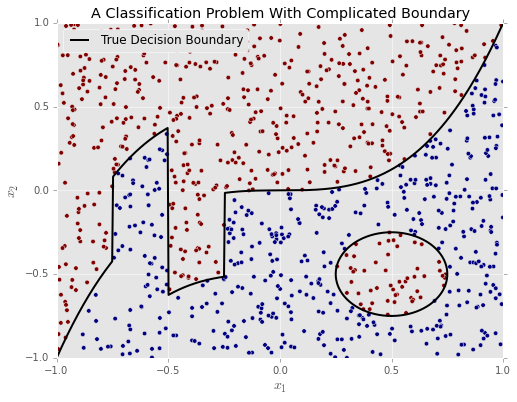
\includegraphics[scale=0.45]{classification-boundary-with-data}
  \end{figure}

\end{frame}
%
\begin{frame}
Gradient boosted logistic regression makes short work of it.

  \begin{figure}
    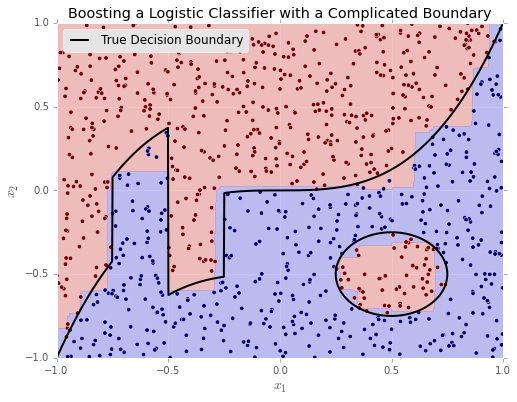
\includegraphics[scale=0.45]{classification-boundary-with-booster}
  \end{figure}

\end{frame}
%
\begin{frame}
Recall our friend logistic regression.

$$ \hat \beta = \argmin_{\beta} \sum_i \left( y_i \nu(\beta, x_i) - \log(1 + e^{\nu(\beta, x_i)}) \right) $$

Where $\nu(\beta, x_i) = \beta_0 + \beta_1 x_{i1} + \cdots + \beta_{M} x_{iM}$.\\~\\ 

The quantity $\nu$ is called the \textit{linear predictor}.\\~\\

In logistic regression it represents the \textit{log odds} of the outcome.
\end{frame}
%
\begin{frame}
Once we have solved for $\hat \beta$, we can make predictions using

$$p(x) = \frac{1}{1 + e^{-(\hat \beta_0 + \hat \beta_1 x_1 + \cdots + \hat \beta_M x_M)}}$$

The predictions can interpreted as \textit{the conditional probability that $y = 1$, given the values of $x$}.

$$ p(x) = Pr(y = 1 \mid x) $$
\end{frame}
%
\begin{frame}
The function we are minimizing in logistic regression is called the \textit{logistic loss}:

$$ L(f, y) = y f - \log(1 + e^{f}) $$

  \begin{figure}
    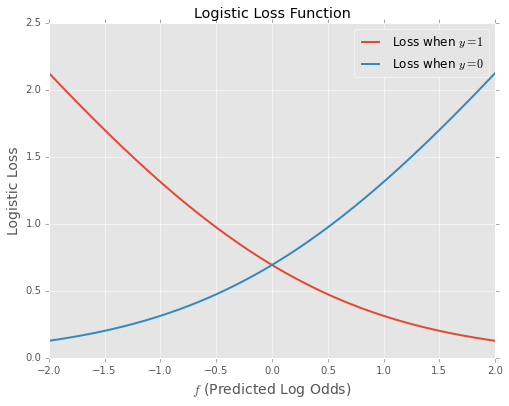
\includegraphics[scale=0.42]{loss-function-logistic}
  \end{figure}
  
\end{frame}
%
\begin{frame}
  \begin{center}
    \textbf{Logistic regression can be solved with gradient descent.}
  \end{center}
\end{frame}
%
\begin{frame}
\textbf{Gradient Boosted Logistic Regression}:\\~\\
Replace the linear predictor in logistic regression 

$$\nu(\beta, x) = \beta_0 + \beta_1 x_1 + \cdots + \beta_{M} x_M$$

With a sum of small regression trees

$$\nu(x) = T_0(x) + T_1(x) + \cdots + T_{\text{max}}(x)$$
\end{frame}
%
\begin{frame}
To fit a Gradient Boosted Logistic Regression, replace the least squares loss function

$$ L(f, y) = \frac{1}{2} \left(f - y \right)^2 $$

With the logistic loss

$$ L(f, y) = y f - \log(1 + e^f) $$

And then use the same gradient boosting technique.

\end{frame}
%
\begin{frame}
\textbf{Note:} There are some subtleties.  I've included the details in an appendix.
\end{frame}
%
\begin{frame}[fragile]
Gradient boosted logistic regression is implemented in sklearn as\\~\\

\begin{lstlisting}[language=python]
from sklearn.ensembles import GradientBoostingClassifier
model = GradientBoostingClassifier()
# Now y must be a np.array of 0 and 1's!
model.fit(X, y)
\end{lstlisting}
\end{frame}
%
\begin{frame}[fragile]
The options to \texttt{GradientBoostingClassifier} are the same as those to \texttt{GradientBoostingRegressor}\\~\\

\begin{lstlisting}[language=python]
GradientBoostingClassifier(loss='deviance',
                           n_estimators=100, 
                           learning_rate=0.1, 
                           max_depth=3,
                           subsample=1.0, 
                           min_samples_split=2, 
                           min_samples_leaf=1, 
                           min_weight_fraction_leaf=0.0,
                           ...)
\end{lstlisting}

And everything we said before generalizes.
\end{frame}
%
\begin{frame}[fragile]
To make predictions use \texttt{predict\_proba}\\~\\

\begin{lstlisting}[language=python]
model.predict_proba(X)
\end{lstlisting}

The \texttt{predict} method returns \textit{class labels} (by comparing the probability to $0.5$), making it much less useful.
\end{frame}
%
\begin{frame}[fragile]{Gradient Boosted AdaBoost}
By using the \texttt{'exponential'} loss, we get the Adaboost algorithm:

\begin{lstlisting}[language=python]
model = GradientBoostingClassifier(loss='exponential')
model.fit(X, y)
\end{lstlisting}

\end{frame}
%
\begin{frame}
The Adaboost algorithm uses labels $y \in \{-1, 1\}$ and minimizes the loss function

$$ L(f, y) = \exp( - y f) $$

  \begin{figure}
    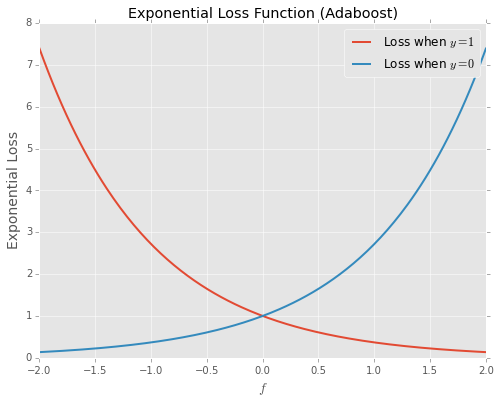
\includegraphics[scale=0.42]{loss-function-adaboost}
  \end{figure}

\end{frame}
%
\begin{frame}
The performance of Adaboost is generally comparable to that of gradient boosted logistic regression

  \begin{figure}
  
    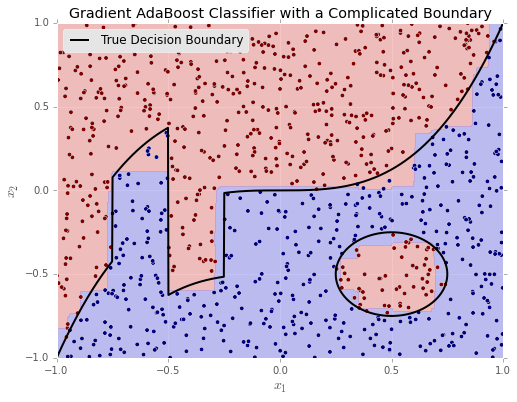
\includegraphics[scale=0.45]{classification-boundary-with-ada-gradient-booster}
  \end{figure}
  
\end{frame}
%
\begin{frame}
In fact, the classification boundaries are \textit{the same}

  \begin{columns}
    \column{.5\textwidth}
    \begin{figure}
      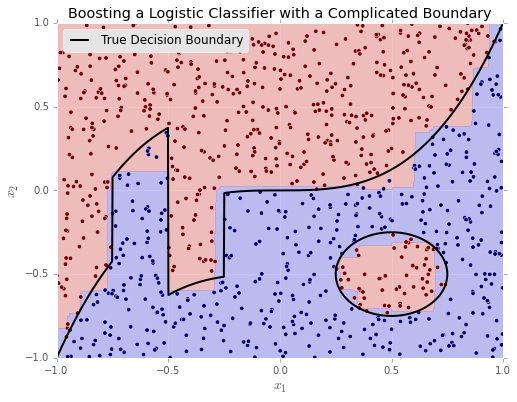
\includegraphics[scale=0.28]{classification-boundary-with-booster}
    \end{figure}
    \column{.5\textwidth}
    \begin{figure}
      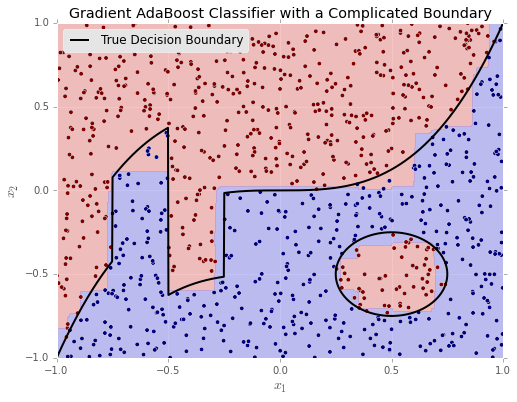
\includegraphics[scale=0.28]{classification-boundary-with-ada-gradient-booster}
    \end{figure}
  \end{columns}
  
\end{frame}
%
\begin{frame}
On the other hand, logistic boosting generally returns better calibrated probabilities, and is less sensitive to outliers.

  \begin{figure}
    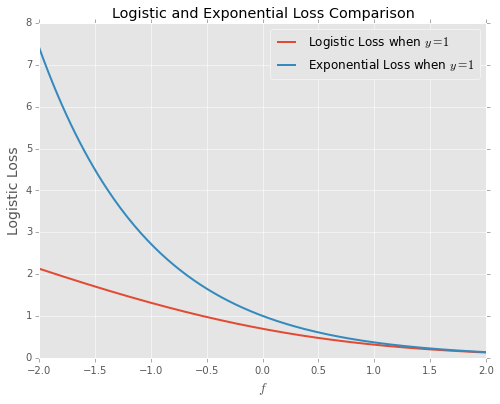
\includegraphics[scale=0.45]{loss-function-comparison}
  \end{figure}
  
\end{frame}
%
\begin{frame}[fragile]
The implementation of Adaboost as a gradient booster is a somewhat recent development.\\~\\

Originally (before the invention of gradient boosting), Adaboost was accomplished by a complicated sample re-weigting scheme.\\~\\
\end{frame}
%
\begin{frame}[fragile]
The traditional Adaboost is included in sklearn as \texttt{AdaBoostClassifier}\\~\\

\begin{lstlisting}[language=python]
model = AdaBoostClassifier(loss='exponential')
model.fit(X, y)
\end{lstlisting}
\end{frame}
%
\begin{frame}[fragile]
Traditional Adaboost is outclassed by gradient boosting, but retains historical and mathematical significance

  \begin{figure}
    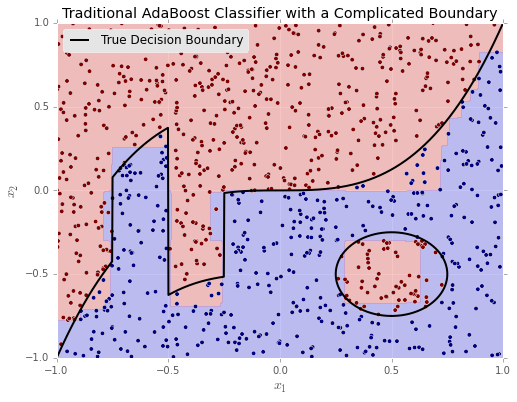
\includegraphics[scale=0.45]{classification-boundary-with-ada-booster}
  \end{figure}
 
\end{frame}
%
\begin{frame}{A Final Comparison of Classification Algorithms}

  \begin{figure}
    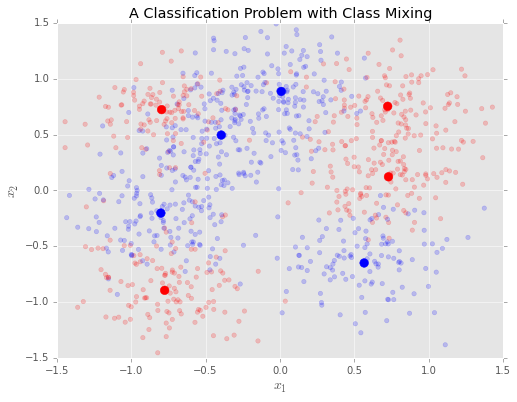
\includegraphics[scale=0.5]{classification-mixed}
  \end{figure}

\end{frame}
%
\begin{frame}

  \begin{figure}
    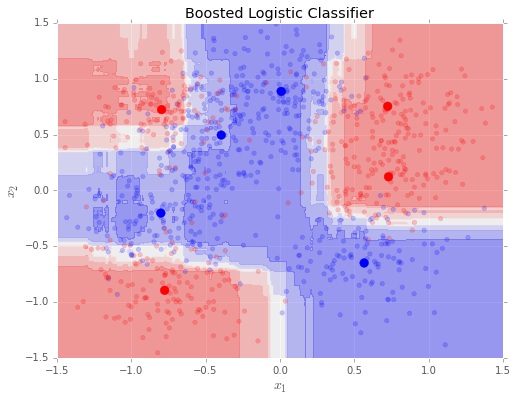
\includegraphics[scale=0.5]{classification-mixed-logistic-boosting}
  \end{figure}
  
\end{frame}
%
\begin{frame}

  \begin{figure}
    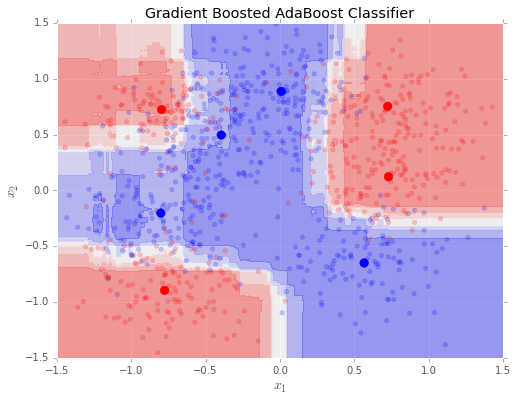
\includegraphics[scale=0.5]{classification-mixed-ada-gradient-boosting}
  \end{figure}
  
\end{frame}
%
\begin{frame}

  \begin{figure}
    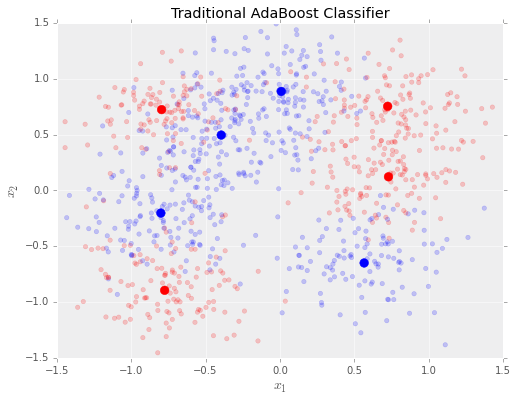
\includegraphics[scale=0.5]{classification-mixed-ada-traditional-boosting}
  \end{figure}
  
\end{frame}
%
\begin{frame}

  \begin{figure}
    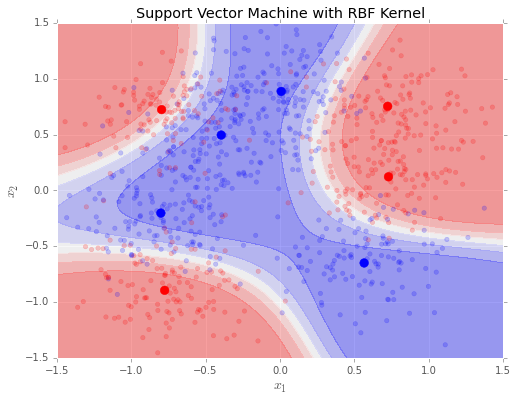
\includegraphics[scale=0.5]{classification-mixed-svm}
  \end{figure}
  
\end{frame}
%
\begin{frame}

  \begin{figure}
    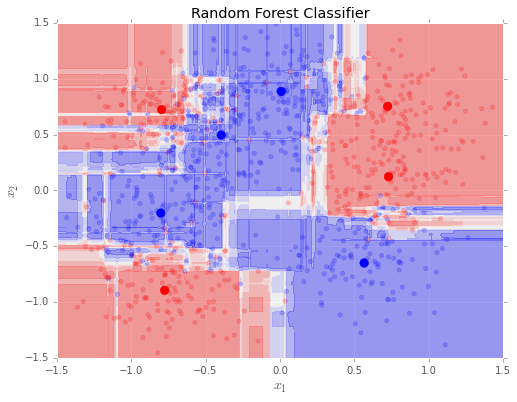
\includegraphics[scale=0.5]{classification-mixed-random-forest}
  \end{figure}
  
\end{frame} % Other Boosting Algorithms
\section{Final Words About Boosting}

\begin{frame}
Gradient Boosting is the best off-the-shelf learning algorithm available today.\\~\\
It effortlessly produces accurate models.\\~\\
\end{frame}
%
\begin{frame}
Nonetheless, it has drawbacks.
\end{frame}
%
\begin{frame}{Drawbacks of Gradient Boosting}
\begin{itemize}

\only<1>{
  \item Boosting creates very complex models.  It can be difficult to extract intuitive, conceptual, or inferential information from them.
}

\only<2>{
  \item Boosting is difficult to explain (maybe you just learned this through experience).  It can be hard to convince business leader to accept such a black box model.
}

\only<3>{
  \item Boosted models can be difficult to implement in production environments due to their complexity.
}

\only<4>{
  \item The sequential nature of the standard boosting algorithm makes it very difficult to parallelize (compared to, for example, random forest).  Recently, there has been great progress (xgboost).
}

\end{itemize}
\end{frame}
%
\begin{frame}{Q\&A}
  \begin{itemize}
    \item Understand the conceptual foundation of Boosting
    \item Understand the algorithm's hyperparameters, and how to tune them.
    \item Understand some basic strategies for interpreting a booster.
    \item Understand the drawbacks of boosting.
    \item Be aware of the possibility of creating your own loss function.
  \end{itemize}
\end{frame}
\end{document}
